\documentclass[a4paper]{article}
\usepackage[T1]{fontenc}
\usepackage[latin1]{inputenc}
\usepackage[italian]{babel}

\usepackage{amsmath,booktabs, graphicx, longtable, wrapfig, subfig, float, rotating}
\usepackage{lipsum, comment}

\begin{document}
\title{Simulazione Evangelizzazione}
\date{ }
\maketitle

\section{Introduzione}
L'ambiente sviluppato simula lo scontro tra differenti fazioni rappresentate da celle, queste simulazioni prendono apertamente ispirazione dagli scontri - sempre frequenti nel passato come nel presente - tra i fedeli delle tre religioni abramitiche; l'interfaccia grafica stessa presenta riferimenti espliciti alla Chiesa Romana, ci� per� non impone all'utente di dover obbligatoriamente giocare dalla parte dei cristiani. I fedeli interagiscono questi fedeli tra loro nella seguente maniera:
\begin{itemize}
	\item Cristiani
		\begin{itemize}
			\item Se un cristiano � a contatto con 3 o pi� cristiani muore.
			\item A contatto con uno o due musulmani un perisce se per� sono pi� di 3
			(compreso) si giunge ad un accordo e il cristiano diviene un apostata.
			\item Come sopra ma non � contemplata la conversione.
		\end{itemize}
	\item Musulmani
		\begin{itemize}
		\item Un musulmano che incontra 3 o pi� musulmani muore.
		\item Se viene incontro a uno o due cristiani perisce, se sono 3 o pi� si converte.
		\item Come prima.
		\end{itemize}
	\item Ebrei
		\begin{itemize}
		\item Se il numero di cristiani � pari a 1 o 2 questi hanno la meglio, se per� il 			numero � maggiore si ha conversione.
		\item Se si incontrano un numero di musulmani tra 1 e 3 questi prevalgono altrimenti
		si ha conversione.
		\item Se il numero di ebrei � 3 o superiore si ha uno scontro interno in cui il
		fedele in minoranza ha la peggio.
		\end{itemize}
\end{itemize}

\section{GUI}
\begin{figure}
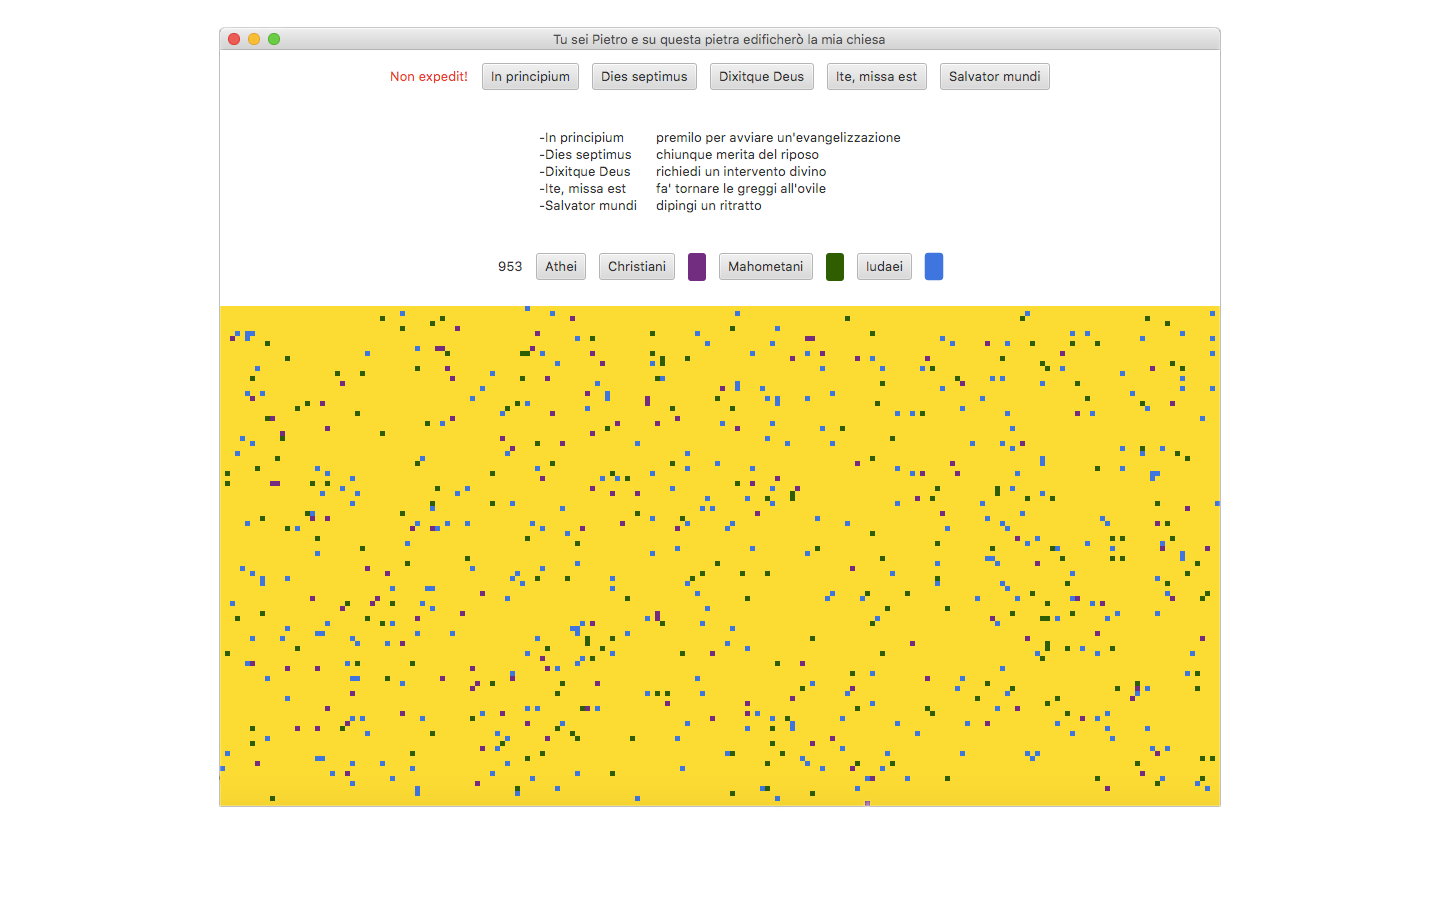
\includegraphics[width=1.3\linewidth]{gui.png}
\end{figure}
Come si pu� vedere in figura l'interfaccia grafica si sviluppa su tre livelli (quattro includendo il testo contenente le istruzioni). In alto si hanno bottoni con differenti funzioni, dei bottoni che permettono la scelta dei fedeli da inserire sul campo e infine un pannello che funziona da tela (non � un oggetto di tipo \texttt{Canvas} ma \texttt{Pane}). Per poter colorare gli elementi grafici � stato usato anche il \texttt{CSS} (i bottoni atomici non potrebbero essere colorati altrimenti).

\section{Codice}
Il codice � diviso in due pacchetti, un pacchetto \texttt{gui} contenente la sola classe \texttt{gui} che gestisce la parte grafica e un pacchetto \texttt{dev} contenente la classe astratta \texttt{Player} con le sue sottoclassi \texttt{Christian}, \texttt{Muslim} e \texttt{Jew} e un'ultima classe \texttt{Util} che contiene variabili che ricorrono spesso sia in \texttt{gui} che in \texttt{dev}. Per gestire il multithreading con l'interfaccia � risultato necessario ricorrere alle classi generiche \texttt{Service} e \texttt{Task} - entrambe implementano l'interfaccia \texttt{Worker} - poich� in \texttt{JavaFX} l'interfaccia grafica � un thread la cui modifica da parte di un altro genera una \texttt{ConcurrentModificationException}, ci� si evita usando un oggetto della classe \texttt{Task} che genera un thread che si distacca dalla normale esecuzione e poi grazie a \texttt{Service} pu� comunicare con l'interfaccia grafica. Per leggere il colore di ogni cella inizialmente si scattava uno snapshot da cui si poteva leggere il colore di un pixel, processo per� troppo lento e due cicli for annidati svolgono il lavoro in maniera pi� efficiente anche grazie all'utilizzo di una \texttt{HashMap} che prende le coordinate di un oggetto e l'oggetto stesso, eliminando dalla lista quegli oggetti che escono dai limiti del campo. \\ L'utilizzo di \texttt{Pane} ha inizialmente causato qualche problema riguardo la gestione della posizione di \texttt{Rectangle}, per ovviare a ci� � stata utilizzata la formula $c = c - (c \mod l)$ con $l$ lunghezza del lato della \texttt{Shape}, portando per� a perdere fluidit� di movimento

\end{document}
